\documentclass{article}
\usepackage[top=3cm,bottom=3cm,left=3cm,right=3cm]{geometry}
\usepackage[utf8]{inputenc}
\usepackage[default]{sourcesanspro}
\usepackage[hidelinks]{hyperref}
\usepackage[acronym]{glossaries}
\usepackage{glossary-inline}
\usepackage{graphicx}
\usepackage{float}

\usepackage{biblatex}
\addbibresource{references.bib}

\makeglossaries
\input{glossary}
\setglossarystyle{inline}

\title{Sentiment140 dataset - Deep learning models}
\author{Dinh \textsc{CôngMinh}, Elie \textsc{Kadoche}, Thomas \textsc{Petiteau}}
\date{15/05/2020}

\begin{document}

\maketitle

\paragraph{Abstract}
We present methods of sentiment analysis from messages from the Twitter with the Sentiment140 dataset.
We insist on the message pre-processing phase, we try a convolution network and a LSTM network. The code can be found \href{https://github.com/XanX3601/deep_sentiment140.git}{here}.
The README.md contains all information concerning the project usage.

\section{Introduction}

Twitter, a public social network, contains tweets from all kinds of sources, making the language used very varied; the data sets provided are further evidence, including a wide range of tweets, from very formal tweets, such as news alerts, to very subjective and often slang tweets, probably from the youngest audience.\\

As such, many difficulties are encountered when trying to classify these tweets, as the variety of vocabulary, format and style is great. Filtering posts, comments and tweets has become a daily problem with public use. Due to the extremely high growth rate in the amount of data produced by social media users, human intervention is not possible in all cases, and therefore a text classifier could easily be useful. The deep learning classifiers and models presented in this project could easily be re-applied to another dataset to regularly discriminate against discriminatory comments.

\section{Dataset}

\subsection{Introduction of Dataset}

Sentiment140 dataset contains approximately 1.6 million tweets that were automatically retrieved with the Twitter API. 
The training set is annotated in two classes (positive and negative) while the test set is annotated at the hand over three different classes (positive, negative and neutral).
For our experiments, we only use the positive and negative classes of the test set.\\

Each line of the file contains a single tweet containing at maximum 140 characters and can contain several sentences (depending on the length). Because the tweets were collected directly on the twitter API, so they can contain HTML addresses, hashtags \# and usernames (preceded by an \@). 

\begin{table}[]
\begin{tabular}{l|l|l|}
\cline{2-3}
\textbf{}                      & \textbf{Training set} & \textbf{Test set} \\ \hline
\multicolumn{1}{|l|}{positive} & 800,000               & 182               \\ \hline
\multicolumn{1}{|l|}{negative} & 800,000               & 177               \\ \hline
\multicolumn{1}{|l|}{neutral}  &                       & 139               \\ \hline
\multicolumn{1}{|l|}{total}    & 1,600,000             & 498               \\ \hline
\end{tabular}
\end{table}

\subsection{Data pre-processing}

After looking at the data, we saw that the sentences contained HTML tags, punctuation... So we started by eliminating the noise to normalize our sentences.
We remove the HTML tags with the BeautifulSoup module. We also remove all the characters which are not letters and therefore, remove all the punctuation from the texts. Because stopwords, by definition, do not provide information to the text, we also eliminate them. All letters need also to be lowercase.

An example after and before our implementation of cleaning:

\begin{verbatim}
x_train[110]
Out[19]: "RT @designplay Goodby, Silverstein's new site: http://www.goodbysilverstein.com/ 
I enjoy it. nice find!"

x_train_clean[110]
Out[20]: 'rt goodby silverstein s new site i enjoy it nice find'
\end{verbatim}

\subsection{Word embedding}

A way of embedding which was used was through GloVe (Global Vectors). GloVe is a model which allows to transform word into vectors, in which similar words are assigned similar vectors. In our project, a pre-trained model was used, which embeds words as 100-dimensional vectors.

\section{Long short term memory (LSTM) Model}

\subsection{Theories}

Recurrent networks (RNN) are a preferred type of architecture for processing sequences by "encoding" iteratively a sequence, using a function $f$ to calculate the following state by
an encoding step: 

$$h_t = f (x_t, h_{t−1})$$

RNNs are struggling to capture long-term dependencies. This is due to the fact that the gradient is very unstable when going back a few steps.
In our project, we will study variants of RNNs, and in particular Long-Short Term Memories (LSTMs).\\

In particular, the LSTMs are defined by an external state $h_t$ (analogous to those of the usual RNNs) and an internal state $C_t$ which represents the "long-term" memory of the network. At each time step, $C_t$ is updated according to the previous internal state $h_{t − 1}$ and the input $x_t$ by specifying what must be "forgotten" from the past and what must be "remembered" for the future. The new external state is calculated from the new internal state. This writing mechanism is based on the notion of a door borrowed from logic, which makes it possible to mask a part of the signal that has little interest. In the case of neural networks, a gate is a continuous function (and not discrete as in logic), often a linear layer followed by an activation sigmoid (which therefore produces an output between $0$ and $1$).

\begin{figure}
  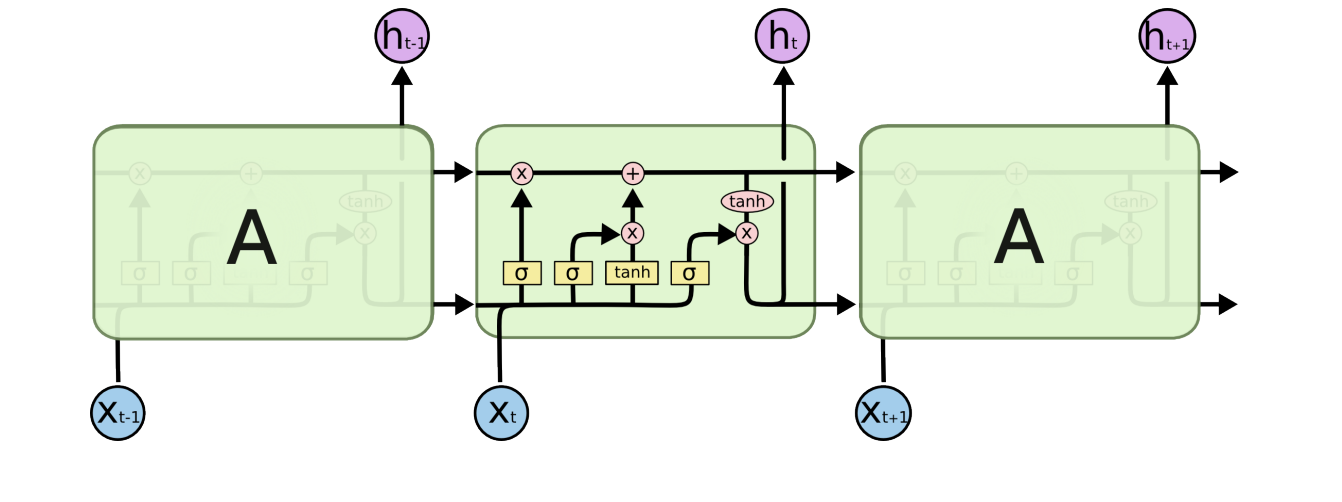
\includegraphics[width=\linewidth]{images/lstm_model.png}
  \caption{LSTM Architecture}
  \label{fig:boat1}
\end{figure}

The evolution of internal and external states is defined by the following equations which rests on three doors (forgetting, entering, and leaving):
\begin{itemize}
    \item Forgotten:
    $$ft = \sigma (W_f .[h_{t - 1}, x_t] + b_f)$$
    \item Entry:
    $$i_t = \sigma (W_i . [H_{t - 1}, x_t] + b_i)$$
    \item Exit:
    $$C_t = f_t \otimes C_{t - 1} + i_t \otimes tanh$$
    \item Update (internal memory):
    $$(W_C . [h_{t - 1}, x_t] + b_C)$$
    \item Output:
    $$o_t = \sigma (W_o . [h_{t - 1}, x_t] + b_o)$$
    \item Exit:
    $$h_t = o_t \otimes tanh (C_t)$$
\end{itemize}

\subsection{Implementation}

\subsubsection{Pre-processing}

After cleaning the data set, we build the vocabulary of the training set using GloVe incorporations. When we build the vocabulary, we initialize the words in the vocabulary using the Gaussian distribution ($unk_init$).

Next, we build vocabulary for the learning set and convert the words to integers. For example we obtain the word corresponding to the integer:

Then it's the construction phase of Iterator. We fill each tweet with the same length to be processed in a batch. The BucketIterator will group tweets of similar lengths for minimized padding in each batch.

\subsubsection{Architecture}

First, we defined the functions $ load \ _train $ and $ load \ _test $ to charge and convert the train or test dataset from numpy to TabularDataset used for our pytorch implementation.

The model LSTM is initialized as below:

\begin{itemize}
    \item vocabulary size;
    \item size of the dense word vectors;
    \item size of the hidden states;
    \item number of classes;
    \item number of multi-layer RNN;
    \item use both directions of LSTM (biLSTM);
    \item dropout probability;
    \item string representing the pad token.
\end{itemize}

We also use an extension of LSTM, BiLSTM. The difference is that BiLSTM has two networks, one accessing
past information in the forward direction while the other one accessing future information in the reverse direction. This architecture can help us achieve a higher accuracy.\\

The model is first built with the Embedding supposedly the first layer of our model. It turns the indexes (positive integers) into dense vectors of fixed size. It is then passed to the LSTM layer, which returns the output and a tuple of the final hidden state and final cell state.\\

Then a Fully-connected layer is applied.\\

We also note a dropout, a method that prevents a neural network from overfitting. So usually it does dropout with a probability of say 0.5. It means at every iteration, only 0.5 of the nodes chosen by random in each layer are working.

\subsubsection{Training}

To set up the training, we use an adam optimizer to update the weights.\\

For the loss function, we use a binary cross entropy with logits.\\

Before starting the training, we defined the $batch\_accuracy$ to returns accuracy per batch, and the $batch\_train$ to to evaluate training loss and accuracy for each iterator.\\

The function $batch\_accuracy$ is simply defined by calculating average correct predictions.\\

The $batch\_train$ is defined to compute the training accuracy and the training loss.  For each batch in the training iterator, we set Zero the gradients, then we Compute the predictions and the loss. We then use this loss to compute gradients. Finally, the gradient step is taken by optimizer. \\

To assess the loss and accuracy of validation and test sets, we created the $ evaluate\_ $ function.\\

The $ evaluate $ function returns the precision of the test dataset. In this function, we divide the dataset into two parts: $ test\_iterator_1 $ which contains 90 \% of the test and $ test\_iterator_2 $ which contains 10 \%. The interest here is to comment on the precision of the model for a larger and smaller data set.\\

The $ train $ function is used to train the model. We have fixed the 4 iterations. In each epoch, we evaluate the loss and accuracy of training and validation. Then we keep the best loss of validation.\\

\subsubsection{Results}

After four epochs, we get $ 71.38 \% $ for training dataset accuracy and  $53.33\%$ for test dataset.\\

LSTM takes words from the transition sequence, from which we removed the punctuation. It may create a little overfit when the sentences get long due to lack of punctuation.

\section*{Conclusion}

We implemented methods related to sentiment analysis with data from the Twitter platform.

\printglossaries
\printbibliography

\end{document}